% !TeX root = RJwrapper.tex
\title{Running basic analyses on Pilot Data}
\author{by Daniela Gawehns and Matthijs van Leeuwen}

\maketitle

\abstract{%
Supplementary Material to ``Social Fluidity in Children's Face-to Face
Interaction Networks''
}

\begin{Schunk}
\begin{Sinput}
library(ggplot2)
\end{Sinput}
\end{Schunk}

\hypertarget{data-cleaning-and-exporting-as-.txt-file}{%
\subsection{Data Cleaning and Exporting as .txt
file}\label{data-cleaning-and-exporting-as-.txt-file}}

The pilot data is included in the package and is formatted into .txt
files with the help of a couple of functions.

\begin{Schunk}
\begin{Soutput}
#> [1] "PilotBeagle"
\end{Soutput}
\begin{Soutput}
#> The following `from` values were not present in `x`: 2041538831
\end{Soutput}
\begin{Soutput}
#> The following `from` values were not present in `x`: 1734935407
\end{Soutput}
\begin{Soutput}
#> [1] 1
#> [1] 2
#> [1] 3
\end{Soutput}
\begin{Soutput}
#> [1] "PilotBeagle"
\end{Soutput}
\begin{Soutput}
#> The following `from` values were not present in `x`: 2041538831
#> The following `from` values were not present in `x`: 1734935407
\end{Soutput}
\begin{Soutput}
#> [1] 1
#> [1] 2
#> [1] 3
\end{Soutput}
\begin{Soutput}
#> [1] "PilotBeagle"
\end{Soutput}
\begin{Soutput}
#> The following `from` values were not present in `x`: 2041538831
#> The following `from` values were not present in `x`: 1734935407
\end{Soutput}
\begin{Soutput}
#> [1] 1
#> [1] 2
#> [1] 3
\end{Soutput}
\end{Schunk}

The created .txt files can be used within the jupyter notebook to
estimate phi and get an overview of several network metrics.

We cannot share the raw data of the data collection with children. We
can however share the derived phi values without a mention of
classrooms, schools or time of the day or time of data collection.

\hypertarget{use-processed-data-to-create-plots}{%
\subsection{Use processed data to create
plots}\label{use-processed-data-to-create-plots}}

Create plots with phi values, as in Fig. 4 of the GEM Paper, showing the
spread of \(\phi\) values.

\begin{Schunk}

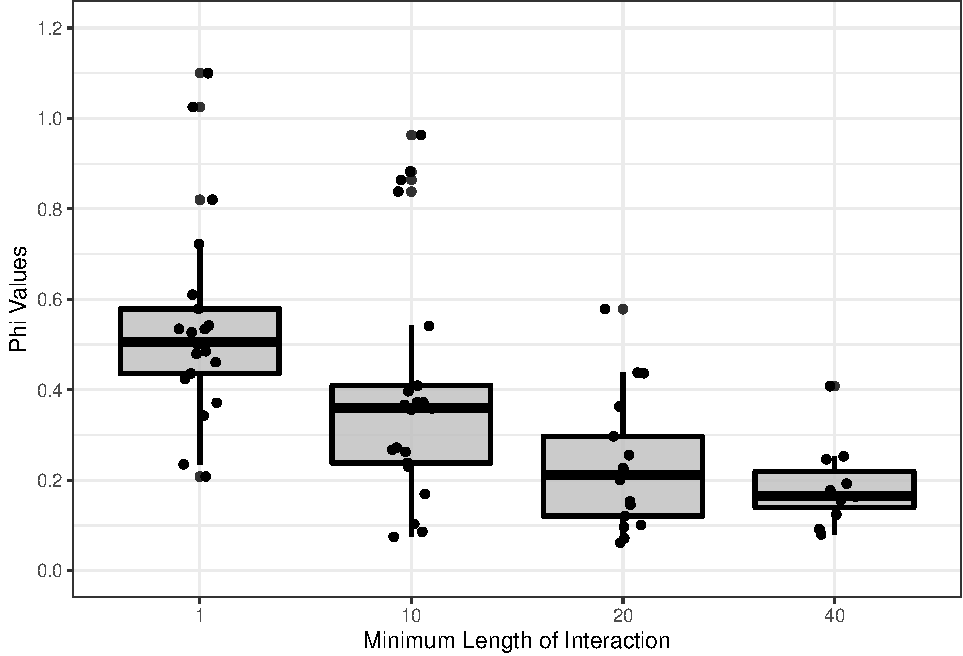
\includegraphics{paper_files/figure-latex/unnamed-chunk-3-1} \end{Schunk}

\bibliography{RJreferences.bib}

\address{%
Daniela Gawehns\\
Liacs Leiden University\\%
line 1\\ line 2\\
%
\url{https://journal.r-project.org}%
\\\textit{ORCiD: \href{https://orcid.org/0000-0002-9079-593X}{0000-0002-9079-593X}}%
\\\href{mailto:author1@work}{\nolinkurl{author1@work}}
}

\address{%
Matthijs van Leeuwen\\
Liacs Leiden University\\%
Niels Bohr Weg 1\\ Leiden, Netherlands\\
Affiliation 2\\%
line 1 affiliation 2\\ line 2 affiliation 2\\
%
\url{https://journal.r-project.org}%
\\\textit{ORCiD: \href{https://orcid.org/0000-0002-9079-593X}{0000-0002-9079-593X}}%
\\\href{mailto:author2@work}{\nolinkurl{author2@work}}
}
